\documentclass[UTF8,a4paper]{ctexart}
%\documentclass[a4paper]{article}
%\usepackage{ctex}
\usepackage{underscore}
\usepackage{multicol}
\usepackage{graphicx}
\usepackage{listings}
\usepackage{amsmath,amssymb,amsfonts}
%\usepackage{url}
\usepackage[colorlinks,linkcolor=blue]{hyperref}
\title{周报}
\author{LiuYan}
\date{\today}
\begin{document}
\section{2019.07.10}
\subsection{Search domain of K}
find a stable pi controller box using interval analysis, then it's possible to find a stable pid controller box in the same way. The box is the search domain of K.
\begin{itemize}
\item (examples/lab7.cpp)the stable pi controller box: depict by vibes(no data but can see subject number:([-100,-10],[-10,0]))\\
\item (examples/in1.cpp)the stable pi controller box: Box after HC4:([-100, -13.66056572379367] ; [-26.74742268041238, 0])\\
\item (examples/in2.cpp)using HC4 to find stable PID controller box: "x before HC4:([-100, 0] ; [-100, 0] ; [0, 100])
 Box after HC4:([-100, -13.45070422535211] ; [-26.77559912854032, 0] ; [0, 20.44925124792014])"
\\
\item choose search domain:([-100,-12],[-27,0],[0,21])
\end{itemize}
%\paragraph{验证}
%by matlab simulation,choose K=(-50,-20,15), the closed-loop system is stable.\\
理解全局最优:由于初始搜索域并不是整个空间,所以不完全是全局最优的。要求:如果要在整个空间寻找全局最优,对计算机计算能力和内存要求过高。
\paragraph{结果}
iter=3117,  size_heap=0,  ymax=44.4284,  uplo= 44.7585\\
iter=3117,  size_heap=0,  ymax=44.4284,  uplo= 44.7585\\
 best bound in: [44.7585,44.8771]\\
 Relative precision obtained on objective function: 0.00264479  [passed]  0.01\\
 Absolute precision obtained on objective function: 0.118691  [failed]  0\\
 precision on variable domains obtained 0.0001  uplo_of_epsboxes 44.7585\\
 best feasible point (-19.7028 ; -0.002648 ; 1.02108)\\
 cpu time used 56.48s.\\
 仿真结果:不稳定,输出y在70s内即发散为脉冲信号。
 \paragraph{扩大搜索域}
 当扩大搜索域为([-100,100],[-100,100],[-100,100]),6分钟后得到best feasible point (50.4389 ; -82.9962 ; -84.8925),仿真依旧不稳定。
 \subsection{PI控制器}
 1.已确定搜索域为([-100, -13.66056572379367] ; [-26.74742268041238, 0]);[0,0].\\
 2.iter=7516,  size_heap=0,  ymax=39.7503,  uplo= 40.1368\\
iter=7516,  size_heap=0,  ymax=39.7503,  uplo= 40.1368\\
 best bound in: [40.1368,40.1518]\\
 Relative precision obtained on objective function: 0.000372783  [passed]  0.01\\
 Absolute precision obtained on objective function: 0.0149679  [failed]  0\\
 best feasible point (-58.7091 ; -3.46578 ; 0)\\
 cpu time used 36.78s.\\
 仿真结果:依旧不稳定。\\
 分析:劳斯判据有问题\\
 \subsection{检查}
 对于特征多项式$a5*s^5+a4*s^4+a3*s^3+a2*s^2+a1*s+a0=0$\\
  \paragraph{wrong routh vector}
  错误的劳斯相量如下:
  \begin{lstlisting}[language={[ANSI]C},numbers=left,numberstyle=\tiny]  
  b1=(a4*a3-a5*a2)/a4;
b2=(a4*a1-a5*a0)/a4;
b3=0;
c1=(b1*a2-a4*b2)/b1;
c2=(b1*a0-a4*b3)/b1;
d1=(c1*b2-b1*c2)/c1;
r1=[a5;a4;b1;c1;d1];
   \end{lstlisting}
    \paragraph{right routh vector}
  由于特征多项式最高次数为n=5次方,所以对应的劳斯相量应该有n+1=6个元素如下:
    \begin{lstlisting}[language={[ANSI]C},numbers=left,numberstyle=\tiny]  
  b1=(a4*a3-a5*a2)/a4;
b2=(a4*a1-a5*a0)/a4;
b3=0;
c1=(b1*a2-a4*b2)/b1;
c2=(b1*a0-a4*b3)/b1;
d1=(c1*b2-b1*c2)/c1;
e1=a0
r1=[a5;a4;b1;c1;d1;e1];
   \end{lstlisting}
   \subsection{PI控制器结果}
   \begin{figure}
  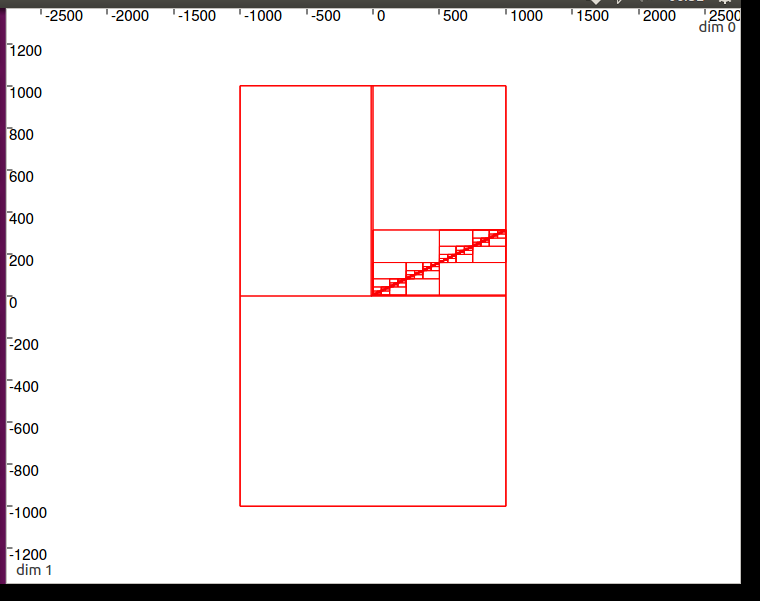
\includegraphics[width=.8\linewidth]{1.png}
  \caption{PI控制器:在([-1000,1000],[-1000,1000])内均无解}
  \label{fig:boat1}
\end{figure}
 \begin{lstlisting}[language={[ANSI]C},numbers=left,numberstyle=\tiny] 
iter=34924,  size_heap=17417,  ymax=8.96088e-317,  uplo= 35.0901
time limit 360s. reached 
 best bound in: [35.0901,inf]
 Relative precision obtained on objective function: inf  [failed]  0.01
 Absolute precision obtained on objective function: inf  [failed]  0
 precision on variable domains obtained 0.0001  uplo_of_epsboxes 36.2078
 no feasible point found 
 cpu time used 360.012s.
\end{lstlisting}
 \subsection{PID控制器结果}
 \begin{lstlisting}[language={[ANSI]C},numbers=left,numberstyle=\tiny]
 iter=1770019,  size_heap=439808,  ymax=6.42317e-317,  uplo= 35.3004
time limit 36000s. reached 
 best bound in: [35.3004,inf]
 Relative precision obtained on objective function: inf  [failed]  0.01
 Absolute precision obtained on objective function: inf  [failed]  0
 precision on variable domains obtained 0.0001  uplo_of_epsboxes 35.3004
 no feasible point found 
 cpu time used 36000s.
\end{lstlisting}
\section{水下机器人建模与鲁棒控制—杨睿}
控制:
\begin{itemize}
\item 被控对象:四自由度(横荡,纵荡,垂荡,艏摇)模型。 鲁棒控制器:艏摇模型。
\end{itemize}
\paragraph{水下航行器定位与制图的卡尔曼与区间方法比较}
在本文中,我们使用卡尔曼滤波器和鲁棒状态观测器来比较水下航行器的定位和映射,使用车辆和位于海底的一组信标之间的仅范围测量。 正如预期的那样,我们表明当我们拥有关于车辆位置和信标的相当好的先验信息时,卡尔曼滤波器表现很好。 基于集合隶属度方法,鲁棒状态观测器证明了在存在异常值的情况下以非常粗略的精度为代价提供一致估计(其中真实解决方案在估计置信域中)的出色能力。 将讨论这种缺乏精确度的根源。
\paragraph{Fuzzy Matrix Contractor Based Approach for Localization of Robots}定位包括找到一些机器人相对于其位置和方向的姿势。 在一组机器人在平面表面上定位的情况下,每个机器人使用可以根据矩阵方程考虑的约束与其他机器人链接。 因此,本章讨论了使用与模糊矩阵承包商相关的角度和距离约束的机器人组的定位。 基于方位距离和方位距离约束的矩阵承包商有助于通过一组机器人有效传播模糊不确定性,以便在没有绝对帧时进行定位。 最后,各种机器人小组已被考虑用于验证拟议的承包商即。 方位角,距离,方位距离和承载距离承包商使用高斯模糊不确定性.\\
\section{2019.07.15}
\section{chapter: Comparison of Kalman and Interval
Approaches for the Simultaneous
Localization and Mapping
of an Underwater Vehicle}
Simultaneous Localization and Mapping 同时定位与地图创建(SLAM)\\
confidence 置信度\\
a fiber optic gyroscope inertial navigation system光纤陀螺惯性导航系统
\begin{itemize}
\item problem: Simultaneous estimate the pose of the vehicle and building the map of its environment.
\item solution: SLAM for localization, 
\end{itemize}
在给水下仪器周围环境建模时估计该仪器姿态时,如何实现两者的同时性是个问题。定位和地图其中一者越精确,另一者也会越精确。对于定位,在水下用SLAM代替GPS进行定位。可以在仪器航行时实时定位。甚至不用先验知识,获得的数据可以直接用于在线校准,节省了时间。SLAM需要对环境进行感知,工具可以是相机,声纳或者其他传感器。本章只讨论声学传感器。(总分为定位和构建地图,引出定位问题为状态估计问题)\\

这种类型的状态估计问题通常用卡尔曼滤波器来求解,因为它是一个经过研究充分,易于理解的状态估计器,已成功用于许多定位问题和SLAM问题。虽然当仪器与信标的初始状态估计良好时,这种方法非常有效,但是当系统没有良好的条件,当出现非线性且得不到良好的初始状态估计时,它的性能会变差。所以卡尔曼滤波器在这些情况下可能会产生高置信度的差估计,并且拒绝较好值得测量,无法将他们和奇异值区分开来,使得检测故障变得棘手。本文提出一种新的集合论方法和卡尔曼滤波器进行比较。集合理论是概率不可知的,有些适用于奇异值有鲁棒性的非线性系统。参考文献8用海上定位比较了卡尔曼滤波器和区间方法。(指出卡尔曼估计的不足)\\

本文比较了并综合了集合论和概率方法去求解水下机器人的SLAM问题。水下定位主要依赖于声音传播的时间为我们提供一些关于水下机器人和一些海标之间的距离。此时集合论方法比较有吸引力。(本文的主要内容)\\

本文组织结构如下。8.2为系统和传感器建模,并考虑了不确定性。8.3将问题描述为一个概率状态估计问题,并用卡尔曼滤波器求解。8.4回忆了区间状态估计的规则和它的优缺点。8.5用真实的数据集合比较了这两种方法。8.6分析了结果,特别讨论了区间估计器缺乏精度的原因。8.7总结本文。\\
\section{2019.08.02}
Matlab的符号运算有所限制,改用Mathematica,需先了解Wolfram语言。
\subsection{Wolfram}
\paragraph{入门}在mathematica的实际操作中,记住三个秘诀即可完成绝大部分功能:\\
1.内置指令首字母大写,采用驼峰原则;\\
2.函数的参数均使用[];\\
3.列表用于储存范围等,使用{};
\paragraph{wolfram语法}
\begin{itemize}
\item $\pi$: Pi
\item $e$: E
\item $A*B$: Dot[A,B]
\end{itemize}
\section{2019.08.06}
\subsection{程序并发,多线程}
1.并行编译: make -j4 file1 file2 file3 file4\\
2.并行运行: 
std::this_thread::sleep_for: 表示当前线程休眠一段时间,休眠期间不与其他线程竞争CPU,根据线程需求,等待若干时间\\
1.我们需要数据并行: 是在数据方面——每个线程在
不同的数据部分上执行相同的操作(第二种方式),被称为数据并行(data
parallelism)\\
2.共享数据
3.互斥锁
4.时间开销项:链接库,
5.多线程需要修改makefile文件为:\\
 \begin{lstlisting}[language={[ANSI]C},numbers=left,numberstyle=\tiny]  
CXXFLAGS += -pthread -fPIC $(COMMON_FLAGS) $(WARNINGS) -std=c++11
NVCCFLAGS += -D_FORCE_INLINES -ccbin=$(CXX) -Xcompiler -fPIC $(COMMON_FLAGS) -std=c++11
LINKFLAGS += -pthread -fPIC $(COMMON_FLAGS) $(WARNINGS) -std=c++11
   \end{lstlisting}
   6.管理线程的函数和类在 <thread> 中声明,而保护共享数据的函数和类在其他头文件中声
明。\\
7.由于线程是有生命周期的,所以须在对象销毁之前就去访问数据,不然单线程一结束,局部对象也会被销毁。thread中的类函数join函数可以确保局部变量在线程结束之后才被销毁。\\
\section{2019.08.07}
\href{http://www.xuetangx.com/courses/course-v1:TsinghuaX+20740084X+2019_T1/about}{《基于linux的c++》}
\paragraph{源代码排版}
\begin{itemize}
\item 递进层次应使用左缩进格式
\item 每行代码不能过长,不能超过 $80$ 个字符
\item 函数代码不超过 $60$ 行
\item 使用空行区分不同功能代码
\item 复合语句书写格式要统一
\item 除非特别必要,否则不要在一行上写多条语句
\item 命名规范要一致
\item 无论采用什么标准,都一定要一直按照该标准进行代码的编辑
\end{itemize}
\section{2019.08.08}
1.普通用户不能添加新的用户,不能删除其他用户的配置文件。
2.如何设置私人文件为他人不可读?  设置文件权限
3.sudo之后的普通用户可以修改所有用户的密码。(很危险)
4..bash_history文件只有本用户和root可读。
5.如何给普通用户加上sudo权限。
\paragraph{iomanip.h}

\end{document}


